\documentclass[14pt]{beamer}
\usepackage{./Estilos/BeamerUVM}
\usepackage{./Estilos/ColoresLatex}
\usepackage{circuitikz}
\usetheme{Warsaw}
\usecolortheme{rose}
%\useoutertheme{default}
\setbeamercovered{invisible}
% or whatever (possibly just delete it)
\setbeamertemplate{section in toc}[sections numbered]
\setbeamertemplate{subsection in toc}[subsections numbered]
\setbeamertemplate{subsection in toc}{\leavevmode\leftskip=3.2em\rlap{\hskip-2em\inserttocsectionnumber.\inserttocsubsectionnumber}\inserttocsubsection\par}
%\setbeamercolor{section in toc}{fg=blue}
%\setbeamercolor{subsection in toc}{fg=blue}
%\setbeamercolor{frametitle}{fg=blue}
\setbeamertemplate{caption}[numbered]

\setbeamertemplate{footline}
\beamertemplatenavigationsymbolsempty
\setbeamertemplate{headline}{}


\makeatletter
\setbeamercolor{section in foot}{bg=gray!30, fg=black!90!orange}
\setbeamercolor{subsection in foot}{bg=blue!30}
\setbeamercolor{date in foot}{bg=black}
\setbeamertemplate{footline}
{
  \leavevmode%
  \hbox{%
  \begin{beamercolorbox}[wd=.333333\paperwidth,ht=2.25ex,dp=1ex,center]{section in foot}%
    \usebeamerfont{section in foot} \insertsection
  \end{beamercolorbox}%
  \begin{beamercolorbox}[wd=.333333\paperwidth,ht=2.25ex,dp=1ex,center]{subsection in foot}%
    \usebeamerfont{subsection in foot}  \insertsubsection
  \end{beamercolorbox}%
  \begin{beamercolorbox}[wd=.333333\paperwidth,ht=2.25ex,dp=1ex,right]{date in head/foot}%
    \usebeamerfont{date in head/foot} \hspace*{2em}
    \insertframenumber{} / \inserttotalframenumber \hspace*{2ex} 
  \end{beamercolorbox}}%
  \vskip0pt%
}
\makeatother

\makeatletter
\patchcmd{\beamer@sectionintoc}{\vskip1.5em}{\vskip0.8em}{}{}
\makeatother
% \usefonttheme{serif}
\usepackage[clock]{ifsym}
\DeclareSIUnit\erg{erg}
\DeclareSIUnit[number-unit-product = {\,}]\cal{cal}

\sisetup{per-mode=symbol}
\resetcounteronoverlays{saveenumi}

% Macro para agregar el logo de UVM en cada slide de la presentación

\addtobeamertemplate{frametitle}{}{%
\begin{tikzpicture}[remember picture,overlay]
\coordinate (logo) at ([xshift=-1.5cm,yshift=-0.8cm]current page.north east);
% \fill[devryblue] (logo) circle (.9cm);
% \clip (logo) circle (.75cm);
\node at (logo) {
\includegraphics[width=2.1cm]{Imagenes/logo_UVM.png}};
\end{tikzpicture}}


\title{\Large{Contenido Cuarto Parcial} \\ \normalsize{Física IV (Área II)}}
\date{}

\begin{document}
\maketitle

\section*{Contenido}
\frame[allowframebreaks]{\frametitle{Contenido} \tableofcontents[currentsection, hideallsubsections]}

\section{Temas a revisar}
\frame{\frametitle{Temas a revisar}\tableofcontents[currentsection, hideothersubsections]}
\subsection{Contenido}

\begin{frame}
\frametitle{Temas a revisar}
Para el último bloque del ciclo escolar de Física IV (Área II), nos enfocaremos en la revisión de los temas de \textocolor{ao}{instrumentación biomédica}, \pause \textocolor{byzantine}{potencial de acción}, \pause \textocolor{red}{seguridad eléctrica} \pause y \textocolor{burgundy}{equipo biomédico}.
\end{frame}


\subsection{Instrumentación biomédica 1}

\begin{frame}
\frametitle{Primer contenido}
\vspace*{-1cm}
\setbeamercolor{item projected}{bg=amber,fg=black}
\setbeamertemplate{enumerate items}{%
\usebeamercolor[bg]{item projected}%
\raisebox{1.5pt}{\colorbox{bg}{\color{fg}\footnotesize\insertenumlabel}}%
}
\begin{enumerate}[<+->]
\item Estetoscopio.
\seti
\end{enumerate}
\begin{figure}
    \centering
    
\includegraphics[scale=0.6]{Imagenes/Instrumentacion_01.jpg}
\end{figure}
\end{frame}
\begin{frame}
\frametitle{Primer contenido}
\vspace*{-1cm}
\setbeamercolor{item projected}{bg=amber,fg=black}
\setbeamertemplate{enumerate items}{%
\usebeamercolor[bg]{item projected}%
\raisebox{1.5pt}{\colorbox{bg}{\color{fg}\footnotesize\insertenumlabel}}%
}
\begin{enumerate}[<+->]
\conti
\item Endoscopio.
\seti
\end{enumerate}
\begin{figure}
    \centering
    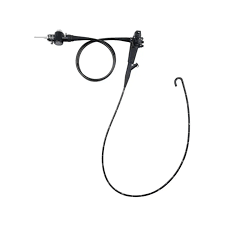
\includegraphics[scale=0.6]{Imagenes/Instrumentacion_02.png}
\end{figure}
\end{frame}
\begin{frame}
\frametitle{¿Endoscopio?}
\begin{figure}
    \centering
    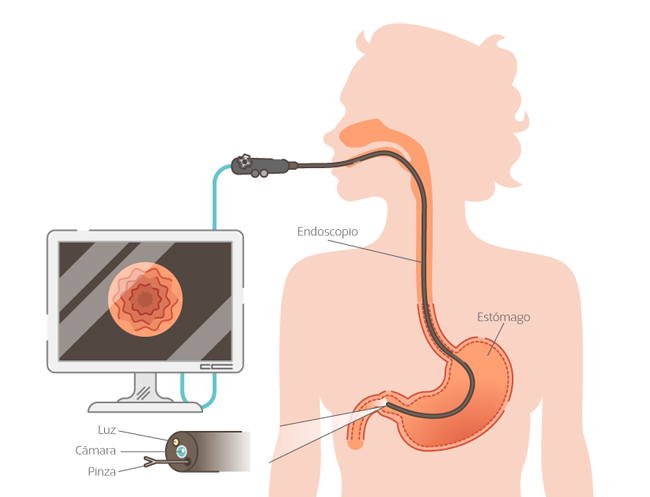
\includegraphics[scale=0.3]{Imagenes/Instrumentacion_03.png}
\end{figure}
\end{frame}
\begin{frame}
\frametitle{Primer contenido}
\vspace*{-1cm}
\setbeamercolor{item projected}{bg=amber,fg=black}
\setbeamertemplate{enumerate items}{%
\usebeamercolor[bg]{item projected}%
\raisebox{1.5pt}{\colorbox{bg}{\color{fg}\footnotesize\insertenumlabel}}%
}
\begin{enumerate}[<+->]
\conti
\item Microscopio.
\seti
\end{enumerate}
\end{frame}
\begin{frame}
\frametitle{Microscopio}
\begin{figure}
    \centering
    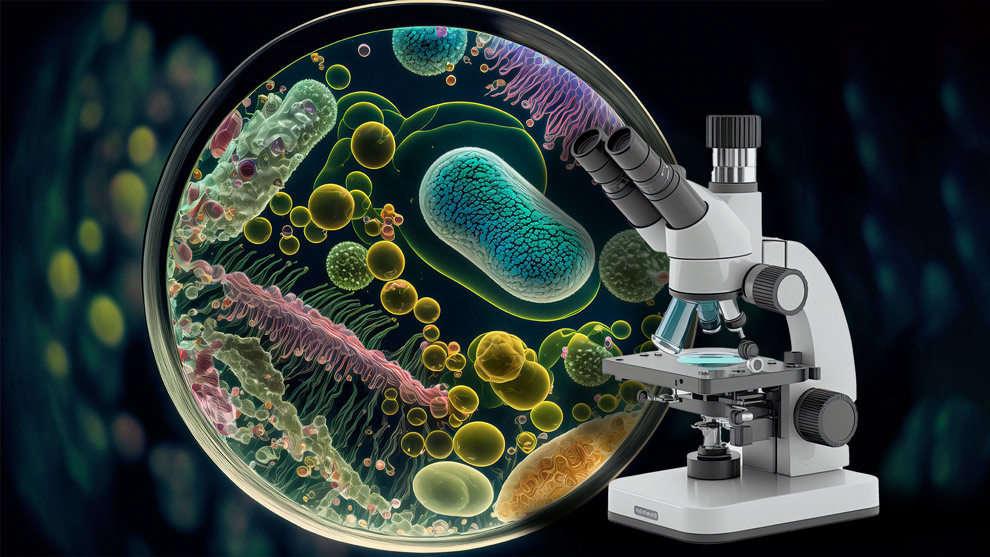
\includegraphics[scale=0.3]{Imagenes/Instrumentacion_06.jpg}
\end{figure}
\end{frame}
\begin{frame}
\frametitle{Primer contenido}
\vspace*{-1cm}
\setbeamercolor{item projected}{bg=amber,fg=black}
\setbeamertemplate{enumerate items}{%
\usebeamercolor[bg]{item projected}%
\raisebox{1.5pt}{\colorbox{bg}{\color{fg}\footnotesize\insertenumlabel}}%
}
\begin{enumerate}[<+->]
\conti
\item Equipo de ultrasonido.
\seti
\end{enumerate}
\end{frame}
\begin{frame}
\frametitle{Ultrasonido}
\begin{figure}
    \centering
    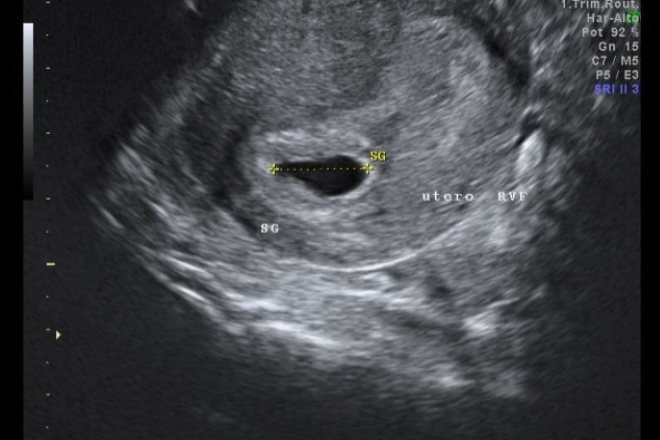
\includegraphics[scale=0.3]{Imagenes/Instrumentacion_05.png}
\end{figure}
\end{frame}
\begin{frame}
\frametitle{Primer contenido}
\vspace*{-1cm}
\setbeamercolor{item projected}{bg=amber,fg=black}
\setbeamertemplate{enumerate items}{%
\usebeamercolor[bg]{item projected}%
\raisebox{1.5pt}{\colorbox{bg}{\color{fg}\footnotesize\insertenumlabel}}%
}
\begin{enumerate}[<+->]
\conti
\item Equipo de rayos X.
\end{enumerate}
\end{frame}
\begin{frame}
\frametitle{Rayos X}
\begin{figure}
    \centering
    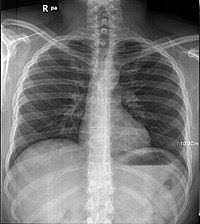
\includegraphics[scale=0.7]{Imagenes/Instrumentacion_07.jpg}
\end{figure}
\end{frame}
\begin{frame}
\frametitle{¿Qué veremos?}
Se revisarán los principios de funcionamiento de estos instrumentos, \pause su aplicación y la relevancia en el diagnóstico y estudios clínicos.
\end{frame}

\subsection{Potencial de acción}

\begin{frame}
\frametitle{¿Qué es el potencial de acción?}
El \textocolor{carmine}{potencial de acción} es un fenómeno eléctrico que ocurre en las células excitables, \pause como las neuronas y las células musculares.
\end{frame}
\begin{frame}
\frametitle{Estudiaremos a la neuronas}
\begin{figure}
    \centering
    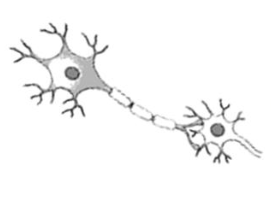
\includegraphics[scale=1]{Imagenes/Potencial_Accion_02.png}
\end{figure}
\end{frame}
\begin{frame}
\frametitle{El potencial de acción}
Es una señal eléctrica rápida y temporal \pause que se propaga a lo largo de la membrana celular \pause y juega un papel fundamental en la \textocolor{cobalt}{comunicación celular} y en la \textocolor{cornellred}{generación de respuestas específicas}.
\end{frame}
\begin{frame}
\frametitle{Midiendo respuesta en la neurona}
\begin{figure}
    \centering
    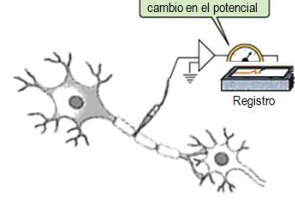
\includegraphics[scale=1]{Imagenes/Potencial_Accion_03.png}
\end{figure}
\end{frame}
\begin{frame}
\frametitle{Midiendo respuesta en la neurona}
\vspace*{-1cm}
\begin{figure}
    \centering
    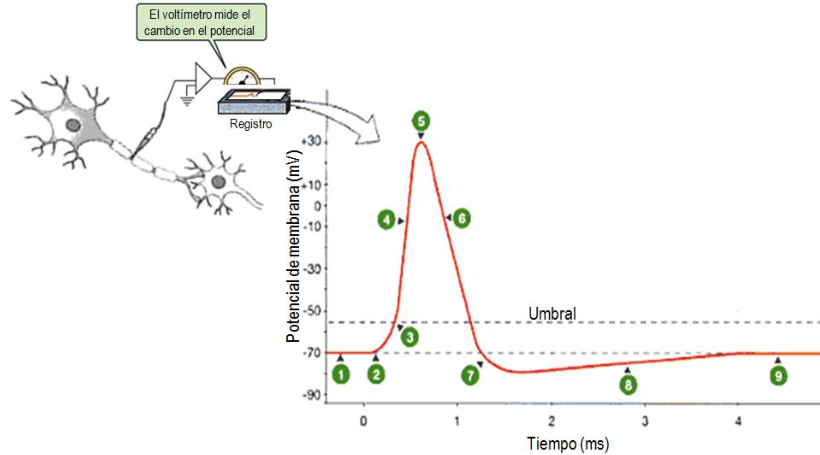
\includegraphics[scale=0.73]{Imagenes/Potencial_Accion_01.png}
\end{figure}
\end{frame}

\subsection{Seguridad eléctrica}

\begin{frame}
\frametitle{La relevancia de la seguridad}
La \textocolor{crimsonglory}{seguridad eléctrica} en el campo de la biomedicina es de suma importancia \pause debido a la \textocolor{armygreen}{naturaleza delicada} de los sistemas biológicos \pause y la necesidad de \textocolor{darkmagenta}{proteger a los pacientes}, \pause al \textocolor{darkred}{personal de salud} \pause y a los \textocolor{denim}{equipos médicos}.
\end{frame}

\subsection{Instrumentación biomédica 2}

\begin{frame}
\frametitle{Más equipo biomédico}
\setbeamercolor{item projected}{bg=electricgreen,fg=black}
\setbeamertemplate{enumerate items}{%
\usebeamercolor[bg]{item projected}%
\raisebox{1.5pt}{\colorbox{bg}{\color{fg}\footnotesize\insertenumlabel}}%
}
\begin{enumerate}[<+->]
\item Esfingomanómetro.
\seti
\end{enumerate}
\end{frame}
\begin{frame}
\frametitle{El esfingomanómetro}
\vspace*{-1cm}
\begin{figure}
    \centering
    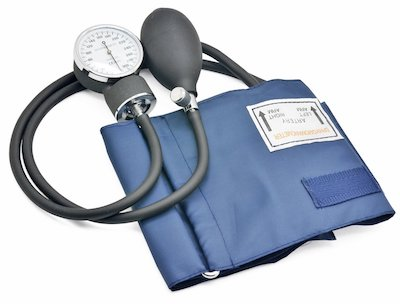
\includegraphics[scale=0.5]{Imagenes/Instrumentacion_08.jpg}
\end{figure}
\end{frame}
\begin{frame}
\frametitle{Más equipo biomédico}
\setbeamercolor{item projected}{bg=electricgreen,fg=black}
\setbeamertemplate{enumerate items}{%
\usebeamercolor[bg]{item projected}%
\raisebox{1.5pt}{\colorbox{bg}{\color{fg}\footnotesize\insertenumlabel}}%
}
\begin{enumerate}[<+->]
\conti
\item Electrocardiógrafo.
\seti
\end{enumerate}
\end{frame}
\begin{frame}
\frametitle{El electrocardiógrafo}
\vspace*{-1cm}
\begin{figure}
    \centering
    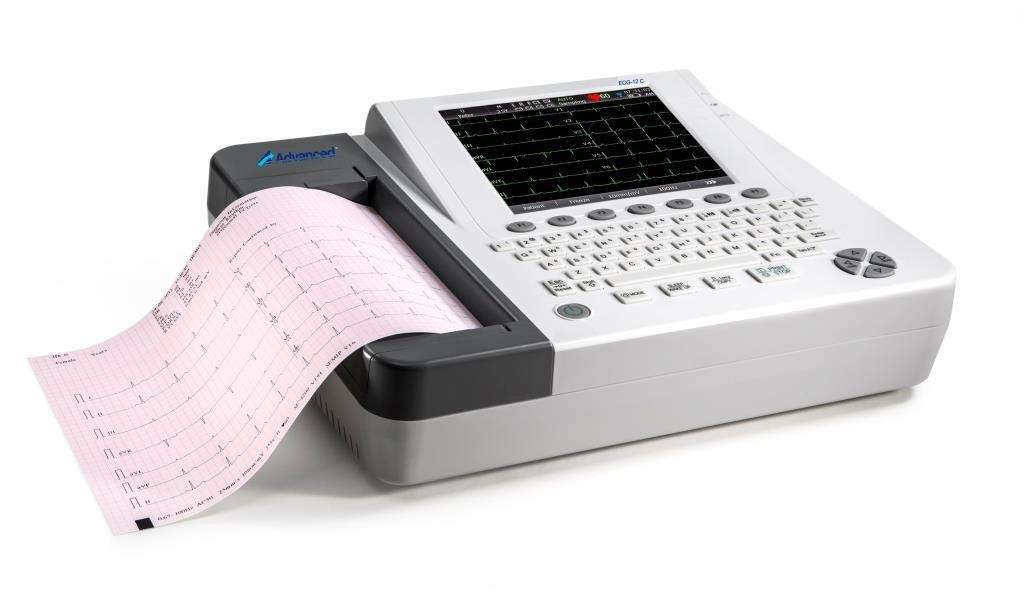
\includegraphics[scale=0.3]{Imagenes/Instrumentacion_09.jpg}
\end{figure}
\end{frame}
\begin{frame}
\frametitle{Más equipo biomédico}
\setbeamercolor{item projected}{bg=electricgreen,fg=black}
\setbeamertemplate{enumerate items}{%
\usebeamercolor[bg]{item projected}%
\raisebox{1.5pt}{\colorbox{bg}{\color{fg}\footnotesize\insertenumlabel}}%
}
\begin{enumerate}[<+->]
\conti
\item Desfibrilador.
\seti
\end{enumerate}
\end{frame}
\begin{frame}
\frametitle{El desfibrilador}
\vspace*{-1cm}
\begin{figure}
    \centering
    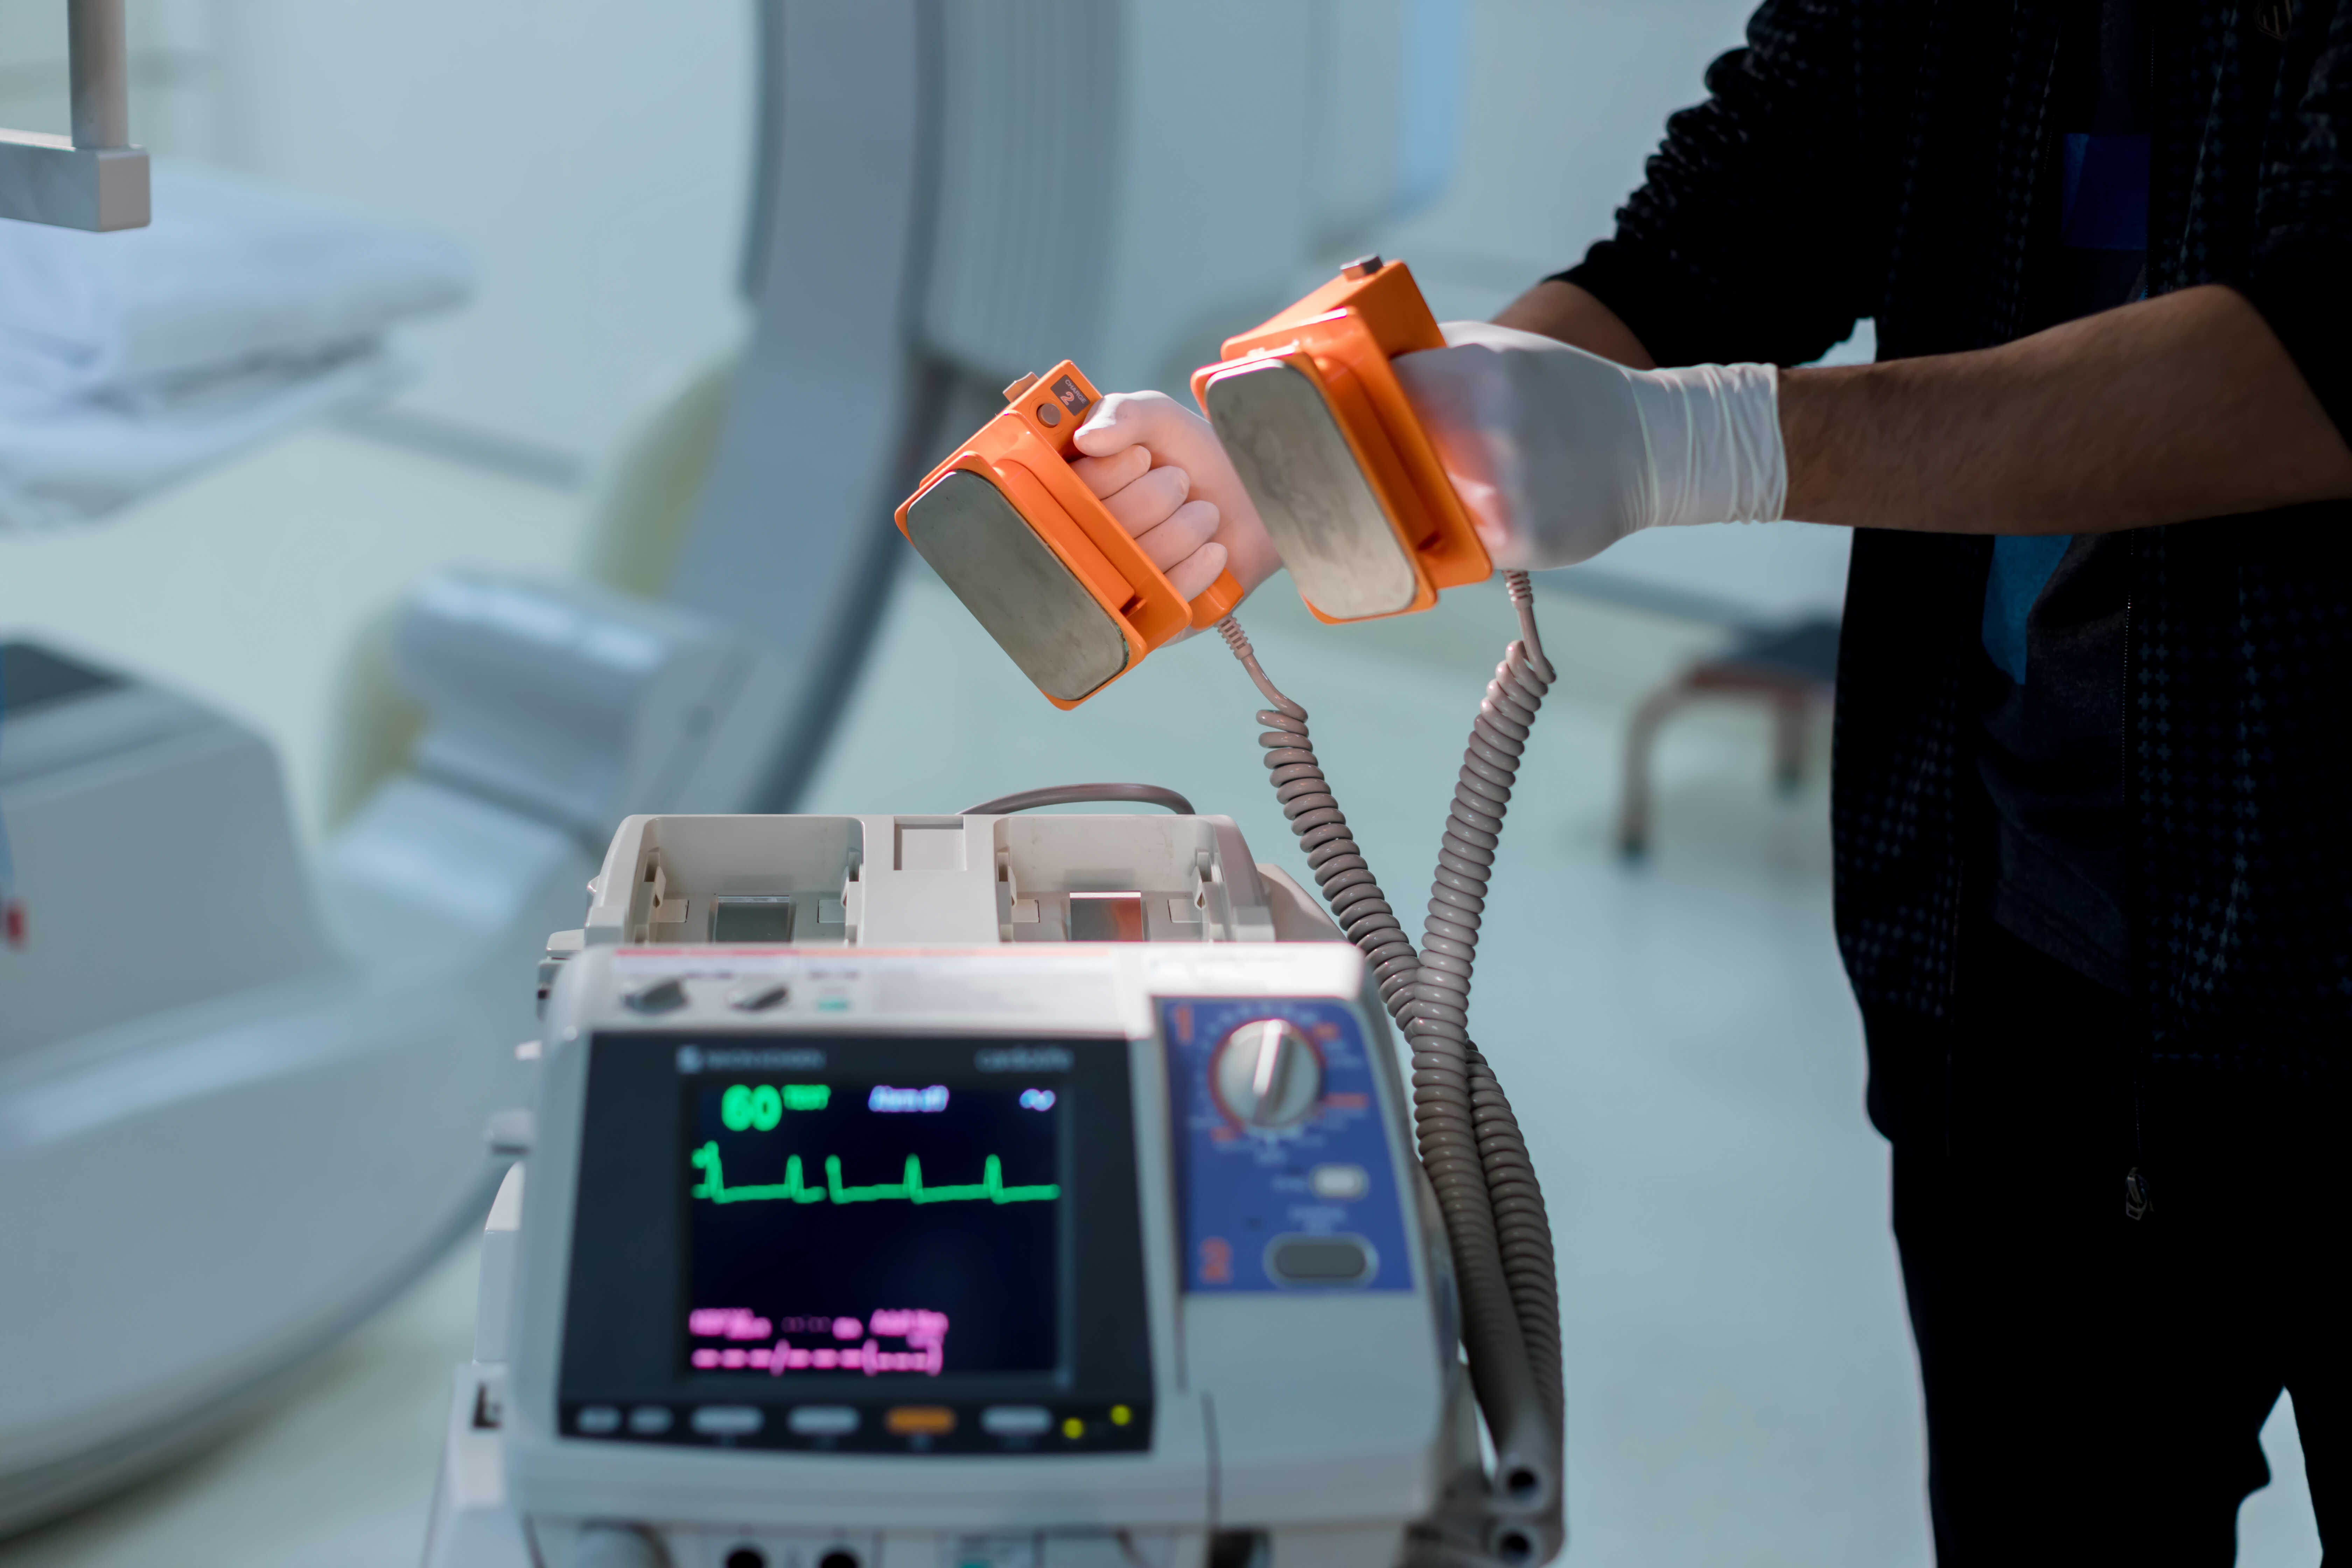
\includegraphics[scale=0.1]{Imagenes/Instrumentacion_10.jpg}
\end{figure}
\end{frame}
\begin{frame}
\frametitle{Más equipo biomédico}
\setbeamercolor{item projected}{bg=electricgreen,fg=black}
\setbeamertemplate{enumerate items}{%
\usebeamercolor[bg]{item projected}%
\raisebox{1.5pt}{\colorbox{bg}{\color{fg}\footnotesize\insertenumlabel}}%
}
\begin{enumerate}[<+->]
\conti
\item Encefalógrafo.
\seti
\end{enumerate}
\end{frame}
\begin{frame}
\frametitle{El encefalógrafo}
\vspace*{-1cm}
\begin{figure}
    \centering
    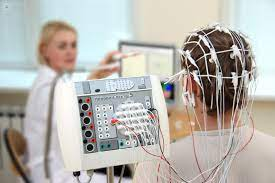
\includegraphics[scale=0.73]{Imagenes/Instrumentacion_11.jpg}
\end{figure}
\end{frame}
\begin{frame}
\frametitle{Más equipo biomédico}
\setbeamercolor{item projected}{bg=electricgreen,fg=black}
\setbeamertemplate{enumerate items}{%
\usebeamercolor[bg]{item projected}%
\raisebox{1.5pt}{\colorbox{bg}{\color{fg}\footnotesize\insertenumlabel}}%
}
\begin{enumerate}[<+->]
\conti
\item Marcapasos.
\end{enumerate}
\end{frame}
\begin{frame}
\frametitle{El marcapasos}
\vspace*{-1cm}
\begin{figure}
    \centering
    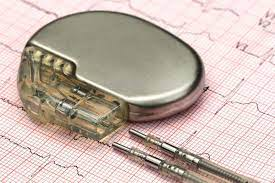
\includegraphics[scale=0.73]{Imagenes/Instrumentacion_12.jpg}
\end{figure}
\end{frame}


\end{document}